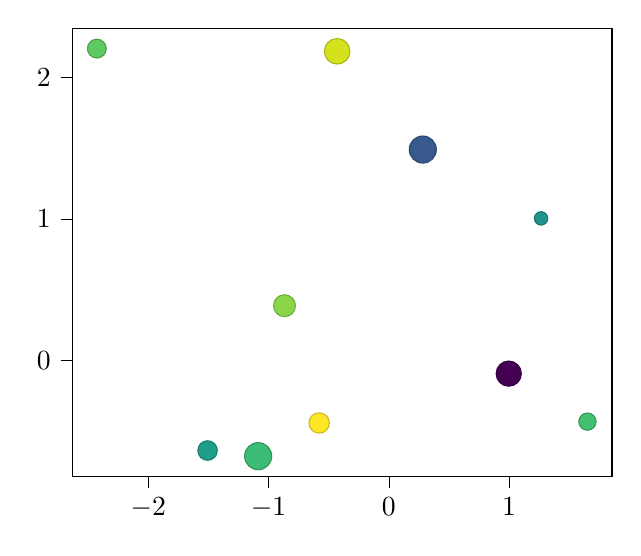
\begin{tikzpicture}

\begin{axis}[
tick align=outside,
tick pos=left,
x grid style={white!69.019608!black},
xmin=-2.630585, xmax=1.8553423,
xtick style={color=black},
y grid style={white!69.019608!black},
ymin=-0.82312696, ymax=2.3501709,
ytick style={color=black}
]
\addplot [
colormap/viridis,
only marks,
scatter,
scatter src=explicit,
scatter/@pre marker code/.append style={/tikz/mark size=\perpointmarksize},
visualization depends on={\thisrow{sizedata} \as\perpointmarksize}
]
table [x=x, y=y, meta=colordata]{%
x  y  colordata  sizedata
-1.0856306 -0.67888615 -0.2556193705305969 4.892567336479345
0.99734545 -0.094708969 -2.7985891054607244 4.548365974103673
0.2829785 1.4913896 -1.771533104509847 4.886673433027043
-1.5062947 -0.638902 -0.6998772345979173 3.5263565080399952
-0.57860025 -0.44398196 0.9274624317585825 3.6807037891241934
1.6514365 -0.43435128 -0.1736356827902158 3.118069713064499
-2.4266792 2.2059301 0.0028459158968110196 3.405493574026048
-0.42891263 2.1867861 0.688222711102285 4.61077361155706
1.2659363 1.0040539 -0.8795363430090519 2.412822212144373
-0.8667404 0.3861864 0.283627323807291 3.9506609882453407
};
\end{axis}

\end{tikzpicture}
